\documentclass[11pt]{article}
\usepackage[a4paper,margin=25mm]{geometry}
\usepackage[T1]{fontenc}
\usepackage{lmodern,amsmath,amssymb,booktabs,graphicx}
\usepackage[hidelinks]{hyperref}
\newcommand{\U}{\mathbf u}
\newcommand{\pr}{\operatorname{pr}}
\newcommand{\dd}{\mathrm d}
\title{Starting a two-dimensional Saint--Venant--Exner extension\\
\large Verified model, rotational reduction and a cubic rotating family}
\author{LieML research calculation}
\date{14 October 2026}
\begin{document}
\maketitle
\begin{abstract}
We start from a checked primary reference for the coupled two-horizontal-
dimensional Saint--Venant--Exner equations. For its frictionless, isotropic
Grass specialization, we independently verify candidate point symmetries,
derive the diagonal-scaling parameter condition, and construct a radial
reduction retaining swirl. At cubic transport, a second symmetry reduces
the radial PDEs to four time-dependent ODEs. Direct Cartesian substitution,
annular balance identities, an exact evolving solution and a small constructed
numerical IVP supply reproducible checks. This is an initial extension
calculation, not a maximal classification, a general well-posedness result,
or a claim of publication novelty.
\end{abstract}

\section{The reference and the exact model being extended}
Fern\'andez-Nieto et al.~\cite{fernandez} display the classical SVE system
in equation (1.1), journal page 116 (PDF page 2), with two horizontal
coordinates, water depth $h_1$, discharge $\mathbf q_1=h_1\U$, sediment
thickness $h_2$ and fixed substrate elevation. The same page states the
Grass law $\mathbf q_b=A_g|\U|^{m_g-1}\U$, $1\leq m_g\leq4$.
We use this introductory classical model, not the paper's later
arbitrary-slope, energy-consistent extension.

Set friction to zero and write $b$ for total Eulerian bed elevation.
The bed remains variable: its slope force is retained. With constant
porosity $0\leq p<1$ and solid-volume transport coefficient $\kappa>0$,
our convention is
\begin{equation}\label{eq:conservative}
\begin{aligned}
 h_t+\nabla\!\cdot(h\U)&=0,\\
 (h\U)_t+\nabla\!\cdot(h\U\otimes\U)
       +\nabla(gh^2/2)+gh\nabla b&=0,\\
 (1-p)b_t+\nabla\!\cdot\bigl(\kappa|\U|^{m-1}\U\bigr)&=0.
\end{aligned}
\end{equation}
The source's Exner flux is normalized by the solid fraction. Thus its
$A_g$ corresponds to $K=\kappa/(1-p)$ here, not to $\kappa$ when the factor
$(1-p)$ is retained. The source and our convention describe the same
balance after this mapping. The bed is measured relative to a fixed datum;
a spatially variable immobile substrate may be included in total $b$.

On the smooth wet region $h>0$, expand the momentum equations and use mass
conservation. The primitive residual vector $E=(E_h,E_u,E_v,E_b)^T$ is
\begin{equation}\label{eq:primitive}
\begin{aligned}
 E_h&=h_t+(hu)_x+(hv)_y,\\
 E_u&=u_t+uu_x+vu_y+g(h+b)_x,\\
 E_v&=v_t+uv_x+vv_y+g(h+b)_y,\\
 E_b&=b_t+K\nabla\!\cdot\bigl((u^2+v^2)^{(m-1)/2}(u,v)\bigr).
\end{aligned}
\end{equation}
In particular the conservative momentum residuals are $uE_h+hE_u$ and
$vE_h+hE_v$; this identity is checked without assuming $E=0$.
It justifies equivalence only where division by $h$ is valid.

Throughout, $g,K>0$ are fixed, solutions are classical and smooth, and
$u^2+v^2>0$ is assumed for arbitrary real $m$. The source-backed range is
$1\leq m\leq4$; other real exponents are a mathematical extension.
At $m=3$ the closure is polynomial and extends to zero velocity.
Numerical examples below use dimensionless variables and coefficients.
No printed scalar Lagrangian equation or its classification is assumed
equivalent to this four-field Eulerian system.

\section{From point generators to verified candidates}
A point field has seven components,
\[
 X=\tau\partial_t+\xi\partial_x+\zeta\partial_y
    +\eta^h\partial_h+\eta^u\partial_u+\eta^v\partial_v+\eta^b\partial_b.
\]
Its first prolongation is obtained by the chain rule, for example
$\eta_i^\alpha=D_i\eta^\alpha-u_j^\alpha D_i\xi^j$.
The script checks identities $\pr^{(1)}X(E)=M E$. These allow nonzero
residual multipliers and prove invariance on $E=0$. They do not solve the
unrestricted determining equations for every possible point field.

For every $m$ on the stated branch, the checked fields are
\begin{equation}\label{eq:candidates}
\partial_t,\quad\partial_x,\quad\partial_y,\quad\partial_b,\quad
R=-y\partial_x+x\partial_y-v\partial_u+u\partial_v,\quad
S=t\partial_t+x\partial_x+y\partial_y.
\end{equation}
Translations and the bed shift give zero prolonged residuals;
$\pr R(E)=(0,-E_v,E_u,0)^T$ and $\pr S(E)=-E$.
Rotating only coordinates while leaving the velocity components fixed
fails: the velocity vector must rotate as well.

To determine what diagonal scaling permits, set
\[
 X_d=a t\partial_t+\beta(x\partial_x+y\partial_y)
       +c(u\partial_u+v\partial_v)+d h\partial_h+e b\partial_b.
\]
Matching the weights of the mass, momentum and bed terms yields
\begin{equation}\label{eq:weights}
 c=\beta-a,\qquad d=e=2c,\qquad d-a=mc-\beta,
 \qquad\boxed{(3-m)c=0.}
\end{equation}
For $m\ne3$ this restricted class leaves only multiples of $S$.
At $m=3$ it also admits
\begin{equation}\label{eq:D}
 D=x\partial_x+y\partial_y+u\partial_u+v\partial_v
                         +2h\partial_h+2b\partial_b.
\end{equation}
This result is recomputed from the 2D equations; it is not imported from
the 1D scalar model. With $\mathcal Q=\nabla\cdot(|\U|^{m-1}\U)$,
the stronger checked off-shell identity is
\begin{equation}\label{eq:defect}
 \pr D(E)-\operatorname{diag}(2,1,1,2)E
            =(0,0,0,(m-3)K\mathcal Q)^T.
\end{equation}
This is a diagonal-scaling stratum and a verified candidate list, not a
maximal point algebra or an unrestricted continuation obstruction.

\section{Rotation removes one spatial variable}
Let $r=\sqrt{x^2+y^2}>0$ and use a local angle $\theta$.
The inverse coordinate Jacobian is $r$, so the polar chart excludes the
origin. Rotation-invariant graphs are
\begin{equation}\label{eq:radial-ansatz}
\begin{aligned}
 h&=h(t,r),& b&=b(t,r),\\
 u&=a(t,r)\cos\theta-w(t,r)\sin\theta,&
 v&=a(t,r)\sin\theta+w(t,r)\cos\theta.
\end{aligned}
\end{equation}
Here $a$ is radial velocity and $w$ is azimuthal velocity (swirl).
Rotation invariance does not require $w=0$.
Substituting with
$\partial_x=\cos\theta\,\partial_r-(\sin\theta/r)\partial_\theta$
and $\partial_y=\sin\theta\,\partial_r+(\cos\theta/r)\partial_\theta$
gives
\begin{equation}\label{eq:radial}
\boxed{\begin{aligned}
 h_t+\frac1r(rha)_r&=0,\\
 a_t+aa_r-\frac{w^2}{r}+g(h+b)_r&=0,\\
 w_t+aw_r+\frac{aw}{r}&=0,\\
 b_t+\frac K r\left[r a(a^2+w^2)^{(m-1)/2}\right]_r&=0.
\end{aligned}}
\end{equation}
The factors $1/r$ record the changing circumference of circles.
Dropping them incorrectly replaces radial flow with planar 1D flow.
The script derives the divergence identity for an arbitrary radial
sediment factor and then specializes it to the Grass law.

In the language of variable compression, $R$ removes the angle from
three independent variables $(t,x,y)$, leaving two, $(t,r)$.
This is still a PDE system. It is not yet an ODE reduction.

\section{A second symmetry at cubic transport gives four ODEs}
At $m=3$, $R$ and $D$ commute. Their projected spatial determinant is
$-(x^2+y^2)$, so their joint projected rank is two on $r>0$.
Their invariant graphs have the form
\begin{equation}\label{eq:cubic-ansatz}
 h=r^2H(t),\qquad a=rA(t),\qquad w=rW(t),\qquad b=r^2B(t).
\end{equation}
An arbitrary constant bed datum $b_*$ may be added to $b$; then use the
conjugate generator $D_{b_*}=D-2b_*\partial_b$ for graph invariance.
The literal $D$ has characteristic $2b_*$ on the shifted bed graph.

For example, mass conservation becomes
\[
 r^2H'+\frac1r\partial_r(r^4HA)=r^2(H'+4AH)=0.
\]
This explicitly explains the coefficient $4$. The corresponding planar
1D quadratic family has coefficient $3$, so copying the old ODE would fail.
All four equations reduce to
\begin{equation}\label{eq:ode}
\boxed{\begin{aligned}
 H'&=-4AH,\\
 A'&=W^2-A^2-2g(H+B),\\
 W'&=-2AW,\\
 B'&=-4KA(A^2+W^2).
\end{aligned}}
\end{equation}
This includes genuinely two-component flow and an evolving bed.
An independent Cartesian reconstruction is
\[
 h=H(x^2+y^2),\quad u=Ax-Wy,\quad v=Wx+Ay,\quad
 b=B(x^2+y^2)+b_*.
\]
Writing the four left sides of \eqref{eq:ode} as
$(F_H,F_A,F_W,F_B)$, direct substitution into \eqref{eq:primitive} gives
\begin{equation}\label{eq:factorization}
 E_h=r^2F_H,\quad E_u=xF_A-yF_W,\quad
 E_v=yF_A+xF_W,\quad E_b=r^2F_B.
\end{equation}
Every coefficient identity in this factorization is checked symbolically.

For general $m$, the same proposed graph instead gives
\[
 E_b=r^2B'+K(m+1)A(A^2+W^2)^{(m-1)/2}r^{m-1}.
\]
The generic powers match only at $m=3$. This does not exclude special
noncubic solutions: for example $A=0$ can give stationary pure swirl.
Outside the source range, $m=-1$ is another zero-divergence special case.
The parameter result concerns a symmetry of the full declared system,
not merely a fortunate individual solution.

\section{An integral, an exact solution, and compatible data}
For $H>0$, the reduced equations imply
\begin{equation}\label{eq:integral}
 \frac{\dd}{\dd t}\left(\frac{W^2}{H}\right)=0.
\end{equation}
On $W\ne0$ with a fixed sign, $W=\operatorname{sgn}(W_0)\sqrt{I H}$
removes one dependent unknown from the ODE system. The branch $W=0$ is
separately invariant. This first integral is distinct from removal of
independent variables by the two PDE symmetries.

There is also an exact evolving family. Set $c_*=\omega^2+1/4$ and take
\begin{equation}\label{eq:exact}
 A=\frac1{2t},\quad W=\frac{\omega}{t},\quad
 H=\frac{c_*(1/(2g)-K)}{t^2},\quad B=\frac{Kc_*}{t^2}.
\end{equation}
It is wet for $t>0$, $r>0$, $2gK<1$. The calculation checks its original
Cartesian PDE residuals exactly. For example $g=1$, $K=1/30$, $\omega=1$
gives $H=7/(12t^2)$ and $B=1/(24t^2)$.
This is a directly verified construction; we make no novelty claim for it.

Restricting a solution to an annulus $r_i\le r\le r_o$ supplies a
constructed verification problem. Initial values and both boundary traces
must be taken from that same solution. They are not independent arbitrary
boundary conditions. The annulus is invariant under rotation; its fixed
radii are not invariant under $D$. Thus $D$ reduces solution graphs before
restriction and is not claimed to be a symmetry of this fixed-domain IBVP.

The water mass and net outward water flux are
\[
 M_h=\frac\pi2(r_o^4-r_i^4)H,\qquad
 \Phi_h=2\pi(r_o^4-r_i^4)AH,\qquad M_h'+\Phi_h=0.
\]
For the evolving bed component,
\[
 M_b=(1-p)\frac\pi2(r_o^4-r_i^4)B,\qquad
 \Phi_b=2\pi\kappa(r_o^4-r_i^4)A(A^2+W^2),\qquad M_b'+\Phi_b=0.
\]
The constant bed datum contributes a constant to $M_b$ and hence no time
derivative. These exact identities check the annular conservation factors
and the porosity convention.

\section{Constructed numerical calculation and scope of the evidence}
We solve \eqref{eq:ode} with $g=1$, $\kappa=0.03$, $p=0.4$, hence $K=0.05$,
\[
 (H,A,W,B)(0)=(1,0.15,0.2,0.05),\qquad 0\le t\le0.2.
\]
These are constructed dimensionless data, not observations and not data
reproduced from a source experiment. DOP853 is compared with an independent
Radau implementation and a looser-tolerance/larger-step DOP853 run.
An additional IVP is compared with \eqref{eq:exact} on $[1,1.2]$.
The calculation records solver settings, sample hashes, first-integral drift,
wet/speed guards and centered-finite-difference defects.
\begin{center}
\begin{tabular}{ll}
\toprule
Diagnostic & Measured value \\
\midrule
DOP853/Radau maximum difference & $1.739\times10^{-12}$ \\
DOP853 step/tolerance comparison & $1.282\times10^{-9}$ \\
Maximum drift of $W^2/H$ & $2.082\times10^{-17}$ \\
Exact-family numerical error & $3.331\times10^{-16}$ \\
Minimum sampled $H$ & $9.783\times10^{-1}$ \\
Minimum sampled speed at $r=1$ & $1.978\times10^{-1}$ \\
Fine centered-difference ODE defect & $7.320\times10^{-6}$ \\
Coarse/fine defect ratio & $3.955\times10^{0}$ \\
\bottomrule
\end{tabular}
\end{center}

\begin{figure}[htbp]
\centering
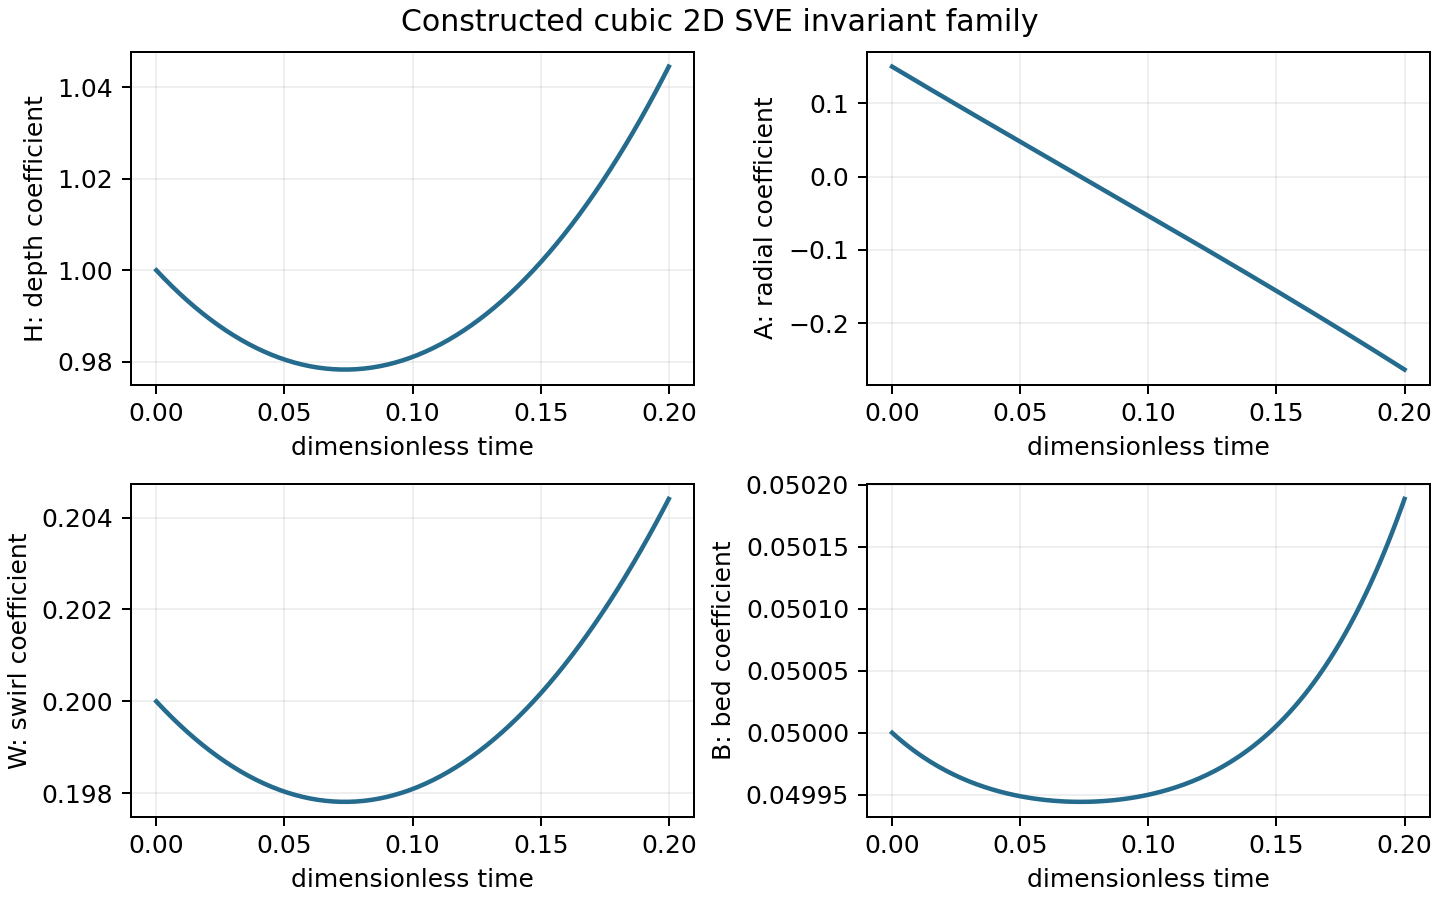
\includegraphics[width=.92\linewidth]{results/profiles.png}
\caption{The constructed rotating-flow IVP. The radial coefficient changes
sign while the angular velocity coefficient stays nonzero. These plotted
curves are numerical solutions of the reduced ODE, not a full 2D simulation.}
\end{figure}

Sampled agreement and finite-difference refinement are consistency evidence,
not a continuous error certificate. The exact family supplies a stronger
special-case residual check, but not stability or well-posedness for general
2D data. Chavarr\'ias et al.~\cite{chavarrias} analyze serious morphodynamic
ill-posedness mechanisms. Their unisize Appendix D still uses a frictional,
low-Froude quasi-steady setting. Its conclusion cannot be transferred here
without checking the hypotheses of our full unsteady frictionless system.

\paragraph{What has been started.}
The new artifact establishes a checked model, candidate symmetries, a
rotation quotient, a cubic ODE family, exact Cartesian and flux certificates,
and a small classical example. The next research gate is the unrestricted
2D determining system, with explicit parameter branches, followed by a
separate analysis of general 2D perturbations and well-posedness. A full 2D
numerical solver, realistic friction/slope closures, arbitrary data, and
ML comparisons remain future work. No source search here proves novelty.

\begin{thebibliography}{9}
\bibitem{fernandez}
E. D. Fern\'andez-Nieto, T. Morales de Luna, G. Narbona-Reina and
J. D. Zabsonr\'e, ``Formal deduction of the Saint-Venant--Exner model
including arbitrarily sloping sediment beds and associated energy,''
\emph{ESAIM: Mathematical Modelling and Numerical Analysis} 51 (2017),
115--145. \url{https://doi.org/10.1051/m2an/2016018}.
Equation (1.1) and the Grass paragraph, p.116, are the model anchors.
\bibitem{chavarrias}
V. Chavarr\'ias, R. Schielen, W. Ottevanger and A. Blom,
``Ill posedness in modelling two-dimensional morphodynamic problems:
effects of bed slope and secondary flow,'' \emph{Journal of Fluid Mechanics}
868 (2019), 461--500. \url{https://doi.org/10.1017/jfm.2019.166}.
Precise consulted pages are recorded in \texttt{SOURCE\_AUDIT.md}; the
warning is model-specific.
\end{thebibliography}
\end{document}
